\chapter{Automatisch uitrollen van databases}
\section{Inleiding}
%Inleiding

\section{IMP: Framework voor installatie}
%Uitleg van IMP
\todo{Te schrijven}
%Uitleg van hoe voor elk systeem

\section{MongoDB}
In deze sectie zal 

\subsection{Werking van MongoDB}
MongoDB heeft gekozen om bij gedistribueerde database op te splitsen in 2 keuzes, een eerste is door middel van \textit{replicaset}s en daarnaast door middel van \textit{shard}ing. 

\paragraph{}Bij \textit{replicaset} is een master-slave configuratie van de MongoDB nodes, met de master benoemd als primary en de slaves als secondary (figuur \ref{fig:mongodb-replicaset}). De data is nog steeds beschikbaar zolang meer als de helft van de nodes beschikbaar zijn. De schrijfoperaties worden eerst naar de primary gestuurd en vervolgens door MongoDB naar de secondaries gesynchroniseerd. Ook leesoperaties worden standaard enkel naar de primary gestuurd maar dit kan aangepast worden in de configuratie. 

Met behulp van een heartbeat houden wordt de status van de verschillende nodes opgevraagd elke 10 seconden en indien de primary niet meer beschikbaar is zal een secondary gestemd worden tot primary (figuur \ref{fig:mongodb-replicaset-vote}). 

\begin{figure}[!htb]
	    \centering
    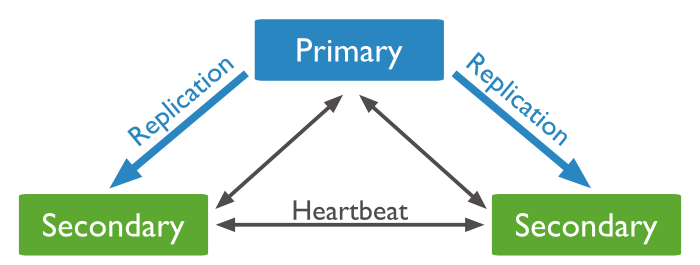
\includegraphics[width=0.7\textwidth]{img/mongodb-replica-set-primary-with-two-secondaries.png}
    \caption{MongoDB: Drie leden van een replicaset met 1 master en 2 slaves. \cite{mongodb-replicaset}}
    \label{fig:mongodb-replicaset}
\end{figure}

\begin{figure}[!htb]
	    \centering
    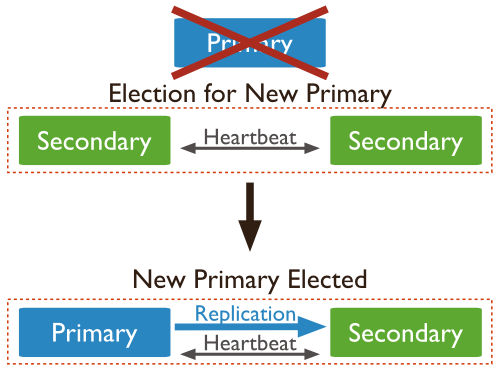
\includegraphics[width=0.7\textwidth]{img/mongodb-replica-set-trigger-election.png}
    \caption{MongoDB: Drie leden van een replicaset met 1 master en 2 slaves. \cite{mongodb-replicaset}}
    \label{fig:mongodb-replicaset-vote}
\end{figure}

\paragraph{} Vervolgens wordt met behulp van \textit{sharding} de data verdeeld over verschillende shards. In productie omgeving wordt aangeraden om een replicaset te nemen als shard maar het is ook mogelijk om een enkele node toe te voegen. 

Voor lees- en schrijfoperaties wordt er hier connectie gemaakt met mongos, dit zijn router nodes die de query naar de nodige shards stuurt. De configuratie van de shards wordt opgeslagen in 1 of 3 configuratie nodes (figuur \ref{fig:mongodb-shards}). 

\begin{figure}[!htb]
	    \centering
    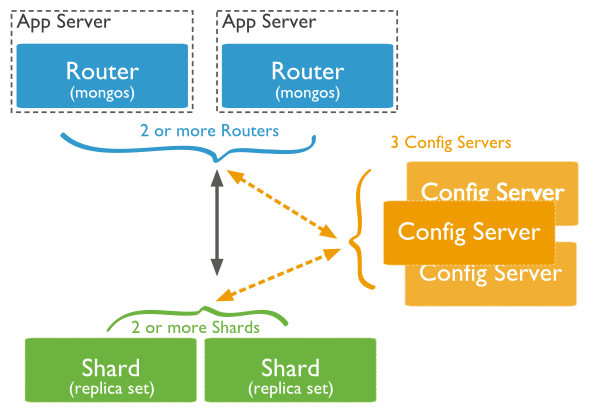
\includegraphics[width=\textwidth]{img/mongo-sharded-cluster-production-architecture.png}
    \caption{MongoDB: Een voorbeeld cluster voor productie met 2 mongos, 3 shards en 3 configuratie servers. \cite{mongodb-shard}}
    \label{fig:mongodb-shards}
\end{figure}

De data wordt verdeeld over de verschillende shards met een door de gebruiker gedefinieerde formule, dit kan door middel van hashing of door het opsplitsen van een waarde in verschillende domeinen. 

\paragraph{} De configuratie van MongoDB is opgesplitst in 2 delen, een configuratiebestand en met behulp van de shell. Als eerste stelt men een configuratiebestand op die aan de instantie basisinformatie meegeeft zoals op welke poort, waar de database op het bestandssysteem op te slaan en welk type de instantie is (enkele node, deel van replicaset, configuratie server of een mongos). 

Het opzetten van de replicasets en sharding verloopt via de shell, met behulp van een commando op een instantie die een deel is van de replicaset kan de replicaset opgezet worden. 
Sharding wordt opgezet door connectie te maken met een mongos en ook hier via commando shards toe te voegen, collecties aan te maken en collecties te verdelen onder shards.

Belangrijk bij sharding is dat bij het opstarten van een mongos al de verschillende configuratie servers meegegeven moeten worden, dit is de enige parameter die meegegeven moet worden in de configuratiebestanden die afhankelijk is van andere instanties. 

\subsection{Uitwerking}


\begin{figure}[!htb]
	    \centering
    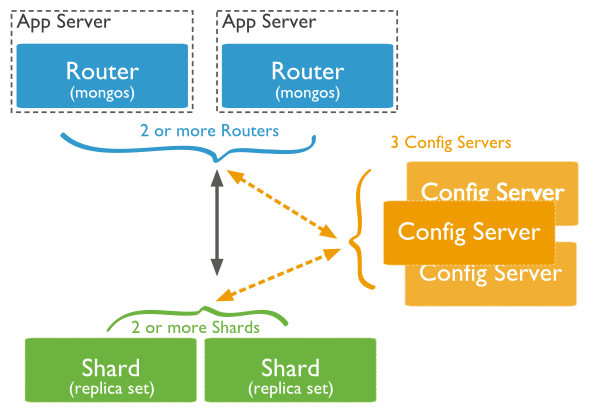
\includegraphics[width=\textwidth]{img/mongo-sharded-cluster-production-architecture.png}
    \caption{MongoDB: Een voorbeeld cluster voor productie met 2 mongos, 3 shards en 3 configuratie servers. \cite{mongodb-shard}}
    \label{fig:mongodb-shards}
\end{figure}
\subsection{Resultaat}